\documentclass{article}

\usepackage{../tex/advi}

\usepackage{color}
\usepackage{graphicx}
\def\adviheader{\noindent
{\bf\Large Active dvi}\\
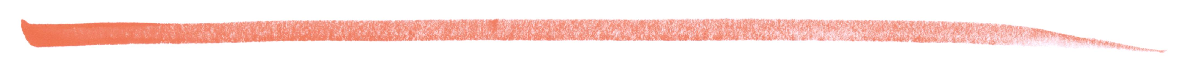
\includegraphics[width=\textwidth]{../tex/bar.jpg.eps}}

\pagestyle{empty}

\definecolor{red}{rgb}{1.0,0.0,0.0}
\definecolor{green}{rgb}{0.0,1.0,0.0}
\definecolor{blue}{rgb}{0.0,0.0,1.0}
\definecolor{c1}{rgb}{1.0,0.0,0.0}
\definecolor{c2}{rgb}{0.5,0.4,0.0}
\definecolor{c3}{rgb}{0.0,0.8,0.0}
\definecolor{c4}{rgb}{0.0,0.4,0.5}
\definecolor{c5}{rgb}{0.0,0.0,1.0}
\definecolor{c6}{rgb}{0.5,0.0,0.5}

\def\keymenu#1{\textcolor{red}{\underline{#1}}}

\def\advifooter{\vbox to 0em{\vbox to \vsize {\vfill
Press: \keymenu{n}ext page \keymenu{p}revious page
\keymenu{\textvisiblespace} next pause%
\hfill{\embedsticky{advianim}{1.56cm}{1.824cm}{animate -geometry !g! -window !p advilogo.anim.gif}}
} \vss}}

\def\adviheader{\noindent
{\bf\Large Active dvi}\\
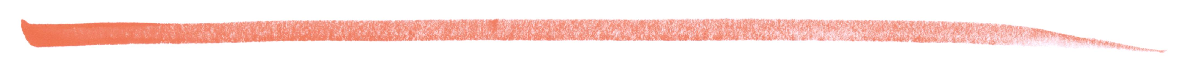
\includegraphics[width=\textwidth]{../tex/bar.jpg.eps}}

\let \Newpage \newpage
\def \newpage {\Newpage \advifooter\adviheader}

\def\adviquitfooter{\vbox to 0em{\vbox to \vsize {\vfill
\hfill \hbox{Press: \keymenu{q} to quit} \hfill~%
} \vss}}

\def\lastpage{\Newpage\adviheader}

\begin{document}

\newpage

\section*{Text movements}

\noindent
Text movements are possible using the \verb"\transbox" \TeX macro.
For instance,

\verb"\transbox{slide from=right}{coming from the right}}"

\noindent move the text {\em coming from the right} from the
right edge of the slide to its correct position into the
page. Variants \verb"right", \verb"left", \verb"top", and
\verb"bottom" of this macro are available.

{
\Huge
\begin{itemize}
\item \textcolor{red}{From \transbox{slide from=right}{right}}
\item \textcolor{green}{From \transbox{slide from=left}{left}}
\item \textcolor{blue}{From \transbox{slide from=top}{top}}
\item \textcolor{cyan}{From \transbox{slide from=bottom}{bottom}}
\end{itemize}
}

\lastpage
\section*{Setting speed of text movements}

\noindent
You can specify the number of steps of the animation with the
extra optional \verb"steps=int" argument. For instance,

\verb"\transbox{slide from=right steps=70}{coming from the right}"

\noindent move the text {\em coming from the right} at a peaceful
pace.

\pause

{
\Huge
\begin{itemize}
\item From \transbox{slide from=right steps=70}{right}
\item From \transbox{slide from=left steps=60}{left}
\item From \transbox{slide from=top steps=70}{top}
\item From \transbox{slide from=bottom steps=100}{bottom}
\end{itemize}
}

\bigskip
\noindent\transbox{slide from=top steps=150}{%
{\begin{minipage}{\textwidth}
\adviheader\\
\end{minipage}}
}

\transbox{slide from=top steps=150}{%
{\begin{minipage}{\textwidth}
\adviquitfooter
\end{minipage}}
}


\end{document}
